---
title :   "Applying Network Science to Reddit: Key Content Detection (Part 2)"
author:   "Rollen S. D'Souza"
date  :   "2018-07-26"
---
Finally we can jump into the analysis!
The purpose of this post is to describe the essential model used for detect key content generators or posts and show what happens when we apply the techniques discussed in the previous post to the \texttt{/r/uwaterloo} subreddit.

\paragraph{The Model}
I could dive straight into the model construction, but I think it is of much greater value to spend some time walking through my thought process.
That way, you can see how I came to my results, and can see the flaws of my approach in all their glory.

\paragraph{The Forest of Posts}
Reddit already has an implicit graph structure embedded in subreddits. One may view a subreddit as a set of submissions, that each are connected to its comments in a tree like fashion. The following diagram depicts the idea.
%
\begin{figure}
    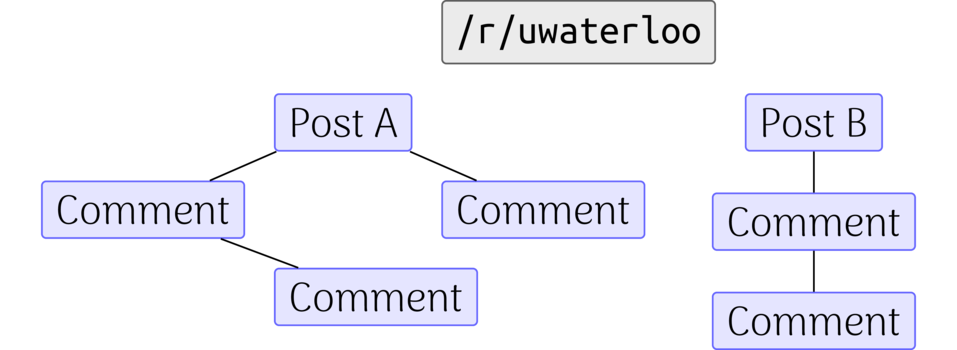
\includegraphics{/images/rna-part-2/reddit-graph.png}
    \caption{Representation of the submission and comment tree hierarchy}
\end{figure}
%
Every subreddit can be structured as a set of (disconnected) trees, whose trees are rooted at the submissions.
The comments are children of the tree, and the leaves are the tail end of any chain of comments.
This structure is formally known as a \textbf{forest} in graph theory.
This implicit structure is natural to any well-versed internet user.
We see it not just on reddit, but on any forum.
HackerNews, general forums, StackOverflow and many other sites take advantage of this structure (and variants of it) as it lends itself to easily organizing discussion around a central (root) piece of content.
This structure brings me to my first assumption.

\textbf{Assumption:} Content is made interesting by its children.

The underlying motivation for this assumption is that content by itself is not what is interesting.
We expect that comments are actually contributing to the content itself.
Note the unidirectionality of this statement.
It implies a direction of "influence."
Looking at the first diagram's first post, we can transform it into,
%
\begin{figure}
    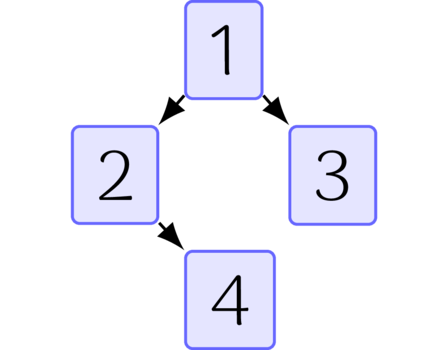
\includegraphics{/images/rna-part-2/reddit-graph-directed.png}
    \caption{Direction of influence from children to parent (comments to submissions)}
\end{figure}
%
The directed edges represent how one node is ``influenced'' by another.
So if Comment A points towards Comment B, Comment A is influenced by Comment B.
Given this transformation, the forest of posts is now a digraph with a forest of out-trees.
This new forest is still not sufficiently interesting.
It only shows how any individual post is affected by its child comments.
What we really want to know is how this post, its comments, and their authors compare to every other piece of content and user active on the containing subreddit.
This motivates an expansion of this graph.

\paragraph{Users Matter}
What makes content interesting is the content creator.
So we would like to add users to the mix! We begin with the simplest of assumptions,

\textbf{Assumption:} Content is made interesting by its author.

Recall that directed edges are our representation of the directed influence of one node to another.
So in this case, content is influenced by its author.
So we will add directed edges from the post or comment to its author,
%
\begin{figure}
    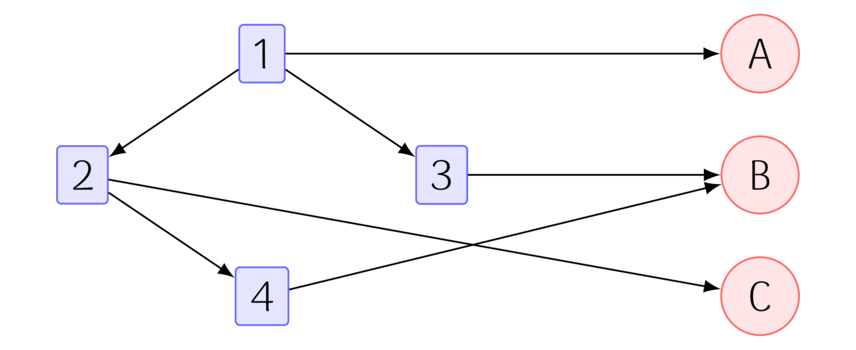
\includegraphics{/images/rna-part-2/reddit-graph-directed-users-1.png}
    \caption{Direction of influence from authors to content.}
\end{figure}
%
Here we have 3 users (A, B, C).
The submission was created by User A.
The comments are created by Users B and C.
Now the structure we have built has some more interesting topology.
For one, the only sinks in this graph (i.e. nodes with no edges going outward) are users.
This means now our trees are rooted in the users active on a subreddit instead of rooted in individual submissions.
This graph could be of interest by itself.
But I chose to add a bit more complexity. Now we take a leap of faith,

\textbf{Assumption:} Authors are influenced by the root submission they comment on.

This assumption has one goal: to model the effect users have on each other.
The idea is that a user would not comment at all unless the post engaged them, positively or negatively.
Note that the assumption is that users are influenced by the root submission and \emph{not} the immediate parent node.
This is a simplification. It may be of value to include this extra edge but I do not.

\paragraph{The Resulting Graph}
So with the above assumption we can transform the example graph into the final form,
%
\begin{figure}
    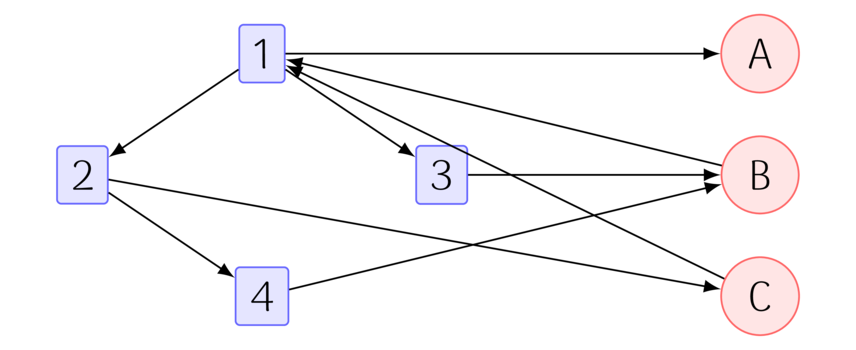
\includegraphics{/images/rna-part-2/reddit-graph-directed-users-full.png}
    \caption{Full example influence digraph.}
\end{figure}
%

\paragraph{The Analysis}
In an earlier post I discussed the Katz Centrality Measure. Recall,

\textbf{Definition:} Let \(A\) be an adjacency matrix for some graph.
Let \(\alpha > 0\) be a sufficiently small constant.
The Katz Centrality measure for node \(i\) is,
\[
  c_i = \sum_{k=1}^{\infty}{ \sum_{j=1}^{n}{ \alpha^k (A^k)_{j,i} } }
\]

This measure when applied to the graph constructed above ranks three effects,
\begin{enumerate}
  \item{
    High scoring submission generate a lot of comments from a large number of users.
  }
  \item{
    High scoring comments generate a lot of comments.
  }
  \item{
    High scoring users generate a lot of posts with a large effect on other users.
  }
\end{enumerate}
So...does it live up to the expectation?
I ran the above analysis on data from the \texttt{/r/uwaterloo} subreddit for dates between November 2017 and February 2018.
This is what we find,
\begin{enumerate}
  \item{supersonic63}
  \item{kw2002}
  \item{\href{https://www.reddit.com/r/uwaterloo/comments/7f2c1d/}{t3\_7f2c1d}}
  \item{\href{https://www.reddit.com/r/uwaterloo/comments/7w0dgv/}{t3\_7w0dgv}}
  \item{\href{https://www.reddit.com/r/uwaterloo/comments/7i045q/}{t3\_7i045q}}
  \item{microwavemasterrace}
  \item{uwsmile}
  \item{\href{https://www.reddit.com/r/uwaterloo/comments/7ld2jb/}{t3\_7ld2jb}}
  \item{mywaterlooaccount}
  \item{honhonhonFRFR}
\end{enumerate}
For those who are not familiar with this subreddit, these are regular users of the community.
These users generate a significant amount of comments and posts.
The submissions --- the links --- characterize the community culture well.
They are links to the admission megathread (discussion about getting into the university) and submissions about the near-God-status Mr. Goose.
One post actually has a comment that made \texttt{/r/bestof}!
This result did surprise me.
I didn't expect it to actually find the users I see most often!
In fact the post \texttt{t3\_7w0dgv} was a pleasant surprise;
I forgot just how much of a stir it caused!

This got me going on another idea.
I could use this technique to find the top most engaging content in a weekly period; this could be presented in a newsletter like fashion!
I'm not sure if I'll do it...but it is a cool application of this algorithm.
